% ============================================================
%  CHAPTER 5 — RESULTS
%  Two top-level sections:
%    1. Preliminary Results  (what is built and measured for TG-1)
%    2. Future Planned Results (what is deferred to TG-2)
% ============================================================

This chapter reports the results achieved in TG-1 and outlines the results
planned for TG-2.  Because the central TG-1 deliverable is the simulator
infrastructure rather than a trained policy, the preliminary results focus on
the simulator's measured throughput, its interface and architecture, and the
status of the prioritized-level-replay sampler.  The planned results describe
the experiments that this infrastructure was built to enable.

% ==================================================================
\section{Preliminary Results}
% ==================================================================

% ------------------------------------------------------------------
\subsection{Simulator Throughput}
% ------------------------------------------------------------------

Throughput is reported as environment steps per second as a function of the
execution path and the number of parallel environments.  All measurements are
taken after \gls{jit} warm-up, so that compilation time is separated from
steady-state rollout speed.  Two hardware configurations were benchmarked,
reflecting the dual development and training setup described in Chapter~4: a
MacBook with an Apple M4 Pro chip, used for CPU execution during development,
and an Ubuntu~22.04 workstation with an NVIDIA RTX~3060 GPU, used for
accelerated experiments.

\subsubsection{Physics Throughput}

The first benchmark isolates the simulator physics from the learning system.
This measurement uses the raw JAX stepping kernel
($\mathrm{jit}(\mathrm{vmap}(\texttt{step}))$), without Gymnasium wrapping,
policy inference, rollout storage, or gradient updates.  No directly comparable
baseline is available in prior VSSS work, because the ODE-based simulators
discussed in Chapter~2 report training duration rather than raw physics-kernel
throughput.  The purpose of this benchmark is therefore not a baseline
comparison, but to show the scale unlocked by expressing the VSSS dynamics as
batched array operations.

Table~\ref{tab:throughput_physics} reports the measured raw physics throughput.
Throughput is computed as
$\text{steps/s} = n_{\mathrm{envs}} n_{\mathrm{steps}} / T$, where $T$ is the
total benchmark latency.  The latency column reports the corresponding
per-call latency of one batched simulator step, i.e., $T/n_{\mathrm{steps}}$.
On the Apple M4 Pro, the JAX backend reaches approximately
$3.0 \times 10^{5}$ steps per second with 256 parallel environments.  On the
RTX~3060, the same batched execution model reaches approximately
$9.1 \times 10^{5}$ steps per second with 1024 parallel environments.

\begin{table}[ht]
    \centering
    \caption{Raw physics throughput and per-call latency of the JAX simulator
    after JIT warm-up.  These measurements isolate the batched stepping kernel
    and do not include learner overhead.}
    \label{tab:throughput_physics}
    \begin{tabular}{llrrr}
        \toprule
        \textbf{Hardware} & \textbf{Execution path} &
        \textbf{\texttt{num\_envs}} & \textbf{Latency/step} &
        \textbf{Steps/s} \\
        \midrule
        Apple M4 Pro & JAX, single environment (jit) & 1 &
            $\sim 20\,\mu\mathrm{s}$ &
            $\sim 5.0 \times 10^{4}$ \\
        Apple M4 Pro & Raw \texttt{jax.vmap} & 256 &
            $\sim 0.85\,\mathrm{ms}$ &
            $\sim 3.0 \times 10^{5}$ \\
        NVIDIA RTX~3060 & Raw \texttt{jax.vmap} & 1024 &
            $\sim 1.13\,\mathrm{ms}$ &
            $\sim 9.1 \times 10^{5}$ \\
        \bottomrule
    \end{tabular}
\end{table}

The physics-only numbers validate the main simulator design choice: for this
domain, the relevant rigid-body kinematics, collisions, and friction model can
be evaluated as a large batch of array operations.  The resulting throughput is
well above the control frequency required by any single VSSS match; the value of
the approach comes from using that headroom to collect experience from hundreds
or thousands of independent games at once.

\subsubsection{Training Throughput}

The second benchmark measures the simulator as used by the current training
stack.  This path includes the Gymnasium-compatible \texttt{VSSVecEnv} wrapper
and, for the end-to-end measurement, a full Stable-Baselines3 \gls{ppo} cycle
with rollout collection and gradient updates.  Unlike the raw physics benchmark,
this result can be compared to the ODE-based training baseline derived in
Chapter~2, Table~\ref{tab:legacy_throughput}, because both quantities describe
environment steps delivered to an RL training loop.

\begin{table}[ht]
    \centering
    \caption{Training-throughput comparison between the prior ODE-based
    ITAndroids baselines and the current simulator stack.  Baseline values are
    derived in Table~\ref{tab:legacy_throughput}; new measurements are taken
    after JIT warm-up.}
    \label{tab:throughput_training}
    \begin{tabular}{llrr}
        \toprule
        \textbf{System} & \textbf{Training path} &
        \textbf{\texttt{num\_envs}} & \textbf{Steps/s} \\
        \midrule
        ODE baseline~\cite{tg_thay} &
            ZeroMQ socket IPC & 1 & ${\approx}63$ \\
        ODE baseline~\cite{master_thiago} &
            merged process with gRPC bridge & 1 & ${\approx}94$ \\
        Apple M4 Pro &
            \texttt{VSSVecEnv} wrapper only & 256 &
            $\sim 1.1 \times 10^{5}$ \\
        Apple M4 Pro &
            Full SB3 \gls{ppo} cycle & 256 &
            $\sim 8\text{--}10 \times 10^{3}$ \\
        NVIDIA RTX~3060 &
            \texttt{VSSVecEnv} wrapper only & 1024 &
            $\sim 9.2 \times 10^{4}$ \\
        \bottomrule
    \end{tabular}
\end{table}

The comparison separates two effects.  First, even the current wrapped
environment delivers orders of magnitude more environment steps per second than
the prior single-instance ODE training setup: approximately
$1.1 \times 10^{5}$ steps per second on the M4 Pro wrapper path and
$9.2 \times 10^{4}$ on the RTX~3060 wrapper path, compared with
${\approx}63$--${\approx}94$ steps per second per simulator instance in the
legacy systems.  Second, when the full \gls{ppo} cycle is included, throughput
falls to approximately $8\text{--}10 \times 10^{3}$ steps per second.  That is
still roughly two orders of magnitude above the Chapter~2 baseline, but it is
far below the raw simulator ceiling.

The remaining gap identifies the next bottleneck.  The \texttt{VSSVecEnv}
wrapper crosses a Python and Gymnasium boundary at every step, converting
between JAX arrays and NumPy arrays.  The full SB3 path adds CPU-bound PyTorch
gradient updates, so the learner cannot stay on the same accelerator as the
simulator.  In other words, the TG-1 simulator removes the original physics and
socket-communication bottleneck, but the current training stack exposes a new
learner-side bottleneck.  The JAX-native training path planned for TG-2 is
designed to close this gap by keeping policy inference, rollout collection, and
optimization on device.

%% FIGURE SUGGESTION 1: A log-scale throughput figure with two panels: raw
%% physics throughput on Mac/RTX, and training throughput against the Chapter 2
%% ODE baselines. This is the single most important figure of TG-1 — it shows
%% both the batching speedup and the remaining learner-side bottleneck.
%% Model it on the throughput-vs-players plot in Smit et al. (2023), Fig. 3.

These results validate the core hypothesis of the work — that expressing VSSS
physics as batched array operations yields throughput far beyond what a
conventional single-instance simulator can achieve — while also precisely
locating the remaining inefficiencies, which the planned JAX-native training
path is designed to eliminate.

% ------------------------------------------------------------------
\subsection{Simulator Interface and Architecture}
% ------------------------------------------------------------------

The second preliminary result is the simulator as a software artifact: a
validated, reusable environment that the learner can call while preserving the
vectorization required for high throughput.

The simulator is organized around a backend-agnostic core with two
interchangeable physics implementations selected at runtime: a reference NumPy
backend and the JAX backend.  The NumPy backend uses \texttt{float64} arithmetic
and a mutable state object, serving as a readable, debuggable reference that
runs anywhere without GPU drivers.  The JAX backend is a pure-functional mirror
of it: its simulation state is an immutable \texttt{NamedTuple} PyTree using
\texttt{float32} arithmetic, which makes it directly compatible with
\texttt{jax.vmap}.  Numerical parity between the two backends was verified to
within an absolute tolerance of $10^{-3}$, so the fast path can be trusted to
reproduce the behavior of the reference.  Physics modelling choices
(Section~\ref{sec:physics_design}, Chapter~4) are shared by both backends;
run-specific training settings are tabulated in
Table~\ref{tab:smoke_config} (Section~\ref{sec:early_training}).

On top of the physics core, the environment exposes a reset–step interface
compatible with batched reinforcement-learning loops.  The batched environment,
\texttt{VSSVecEnv}, runs $N$ independent matches in parallel by applying
$\mathrm{jit}(\mathrm{vmap}(\texttt{step}))$ to a single batched state, and is
registered through the Gymnasium vectorized-environment API.  Auto-reset follows
Gymnasium's next-step convention: a goal triggers an in-episode kickoff, while
episode truncation resets the environment on the following step.  A thin adapter
bridges this Gymnasium-native interface to the Stable-Baselines3 vectorized
protocol, allowing SB3's \gls{ppo} to train on the simulator without any change
to its internals.

The per-step data flow is:
%
\begin{enumerate}
    \item initialize (or reset) a batch of game states;
    \item run policy inference for the controlled team in each environment;
    \item step the batched physics on device;
    \item compute observations, rewards, and termination flags;
    \item accumulate transitions for the \gls{ppo} update.
\end{enumerate}
%
The observation is a 46-dimensional vector per environment (4 ball features and
$6 \times 7$ robot features, all normalized), and the action is a 6-dimensional
vector of normalized left/right wheel speeds for the three controlled robots,
denormalized to physical units inside the backend.  These observation and action
constructions are factored as swappable functions, which keeps the interface
forward-compatible with the per-robot egocentric observations needed for the
multi-agent formulation planned in TG-2.

The robustness of this interface is supported by an automated test suite of 174
unit tests (with 4 GPU-specific tests skipped in the absence of a GPU) covering
physics correctness, backend parity, Gymnasium API compliance, batched
stepping and auto-reset, and the SB3 adapter protocol.  The preliminary TG-1
result is therefore both a software artifact and an architectural validation:
the simulator is straightforward to call from a learner while preserving the
vectorization that the throughput results depend on.

%% FIGURE SUGGESTION 2: An architecture/data-flow diagram showing the backend
%% resolver selecting numpy/jax, the batched SimState flowing through
%% jit(vmap(step)), and the VSSVecEnv → SB3 adapter → PPO learner path. Mirror
%% the "processes communication schema" style used in the prior ITAndroids TGs,
%% but for an on-device loop rather than a socket loop — the contrast makes the
%% architectural contribution legible at a glance.

\begin{figure}[h]
    \centering
    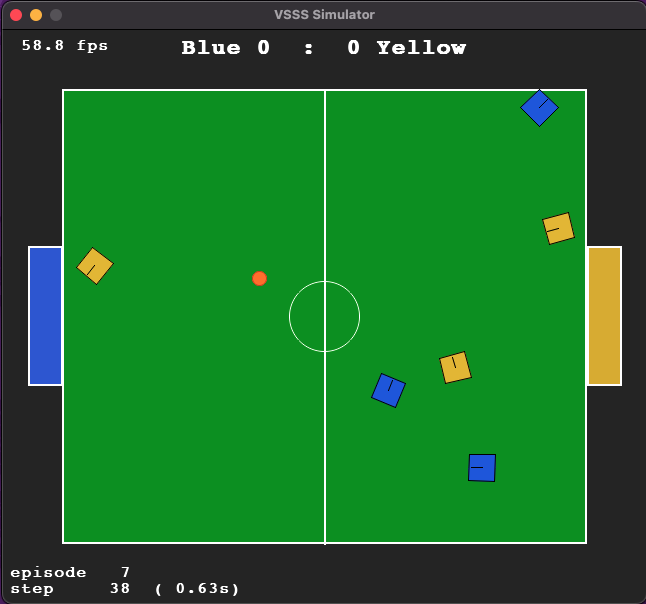
\includegraphics[width=0.8\textwidth]{Cap5/pygame_window.png}
    \caption{Pygame window showing a 3v3 match with the oriented-bounding-box robot shapes, direction indicators, and HUD.}
    \label{fig:pygame_window}
\end{figure}

% ------------------------------------------------------------------
\subsection{Prioritized-Level-Replay Sampler}
% ------------------------------------------------------------------

The third preliminary result concerns the prioritized-level-replay sampler,
which in TG-1 is established at the level of design and supporting
infrastructure rather than full evaluation.

The mechanism that the sampler will hook into is already in place.  Episode
initialization is controlled by a pluggable \texttt{InitMode}, currently
offering a standard kickoff formation (with small random jitter) and a fully
randomized mode that places robots and the ball uniformly across the field.
Both backends implement randomized reset, and the JAX implementation is
\texttt{vmap}-ready, so a batch of distinct initial configurations can be
generated on device in a single call.  Critically, the initialization interface
was designed to accommodate a future selector mode, in which an external model
supplies the placement distribution rather than a fixed rule — this is exactly
the insertion point the \gls{plr} sampler requires.

For TG-1, the contract the sampler must satisfy is defined: it receives
per-scenario statistics from completed rollouts, updates a priority for each
stored scenario from the magnitude of the value-prediction error, and returns a
new batch of initial states biased toward high-priority scenarios while
retaining enough exploration to avoid collapsing onto a narrow set.  The TG-1
deliverable is the demonstration that this contract is compatible with the
batched simulator interface — that scenarios can be stored, scored, and
resampled without breaking vectorization.  Quantitative sample-efficiency
results, in particular learning curves against uniform initialization, are
deferred to TG-2.

% ------------------------------------------------------------------
\subsection{Early Training Validation}
\label{sec:early_training}
% ------------------------------------------------------------------

A final preliminary result is an end-to-end training smoke test confirming that
the \gls{ppo} loop runs correctly on the new simulator.  Using the batched
environment through the SB3 adapter, a Stage-1 configuration (the controlled
team alone, against stationary opponents) was trained with the shaped reward
described in Chapter~4: the sparse $\pm 1$ goal signal augmented by a small
dense term proportional to the ball's forward progress, with the shaping
coefficient set so that its total episodic contribution cannot exceed a single
goal event.  Training runs are tracked with MLflow, logging per-generation mean,
minimum, and maximum reward together with episode length.
Here, one generation denotes one complete episode rollout in each parallel
environment; for these runs, with 256 environments and a 300-step episode cap,
one generation equals $256 \times 300 = 76{,}800$ environment transitions.

The purpose of these early training experiments is not to produce a competitive
policy but to confirm that rollout collection, advantage estimation, optimization,
and checkpointing operate together correctly on the new infrastructure.
Table~\ref{tab:smoke_config} lists every setting that differs from the
simulator defaults or that is shared across both runs; the physics contract
(Table~\ref{tab:physics_design}, Chapter~4) and observation layout
(Table~\ref{tab:obs}) apply unchanged unless noted.
Both runs were executed on a MacBook with an Apple M4 Pro chip
(\texttt{scripts/smoke.py}, batched JAX backend via \texttt{VSSVecEnv}).
Any learning curve reported at this stage should be read as a functional
validation rather than a performance result.

\begin{table}[ht]
    \centering
    \caption{TG-1 smoke-test configuration
    (\texttt{scripts/smoke.py}).  Rows marked ``default'' use
    \texttt{vsss\_sim.config} or SB3 defaults unless overridden on the CLI.}
    \label{tab:smoke_config}
    \small
    \begin{tabular}{p{0.36\linewidth}p{0.22\linewidth}p{0.34\linewidth}}
        \toprule
        \textbf{Parameter} & \textbf{Value} & \textbf{Source} \\
        \midrule
        \multicolumn{3}{l}{\textit{Environment (both runs)}} \\
        Parallel environments     & $256$ & \texttt{--num-envs} \\
        Physics backend           & JAX (batched) & \texttt{VSSVecEnv} \\
        Controlled team           & Blue ($6$ actions) & \texttt{VSSEnv} \\
        Opponent policy           & Stationary & \texttt{opponent\_policy} \\
        Episode cap               & $300$ steps ($5$\,s) & \texttt{--max-episode-steps} \\
        Default episode cap       & $1200$ steps ($20$\,s) & \texttt{MAX\_EPISODE\_STEPS} (not used) \\
        Control frequency         & $60$\,Hz, $4$ sub-steps & \texttt{FPS}, \texttt{SUB\_STEPS} \\
        Reward                    & Eq.~\eqref{eq:reward}, $\beta=0.10$ & \texttt{BALL\_FORWARD\_REWARD\_COEF} \\
        Observation               & $\mathbb{R}^{46}$ (Table~\ref{tab:obs}) & default \\
        \midrule
        \multicolumn{3}{l}{\textit{PPO / SB3 (both runs)}} \\
        Algorithm / policy        & PPO, \texttt{MlpPolicy} & \texttt{PARAMS} \\
        Learning rate             & $3\times 10^{-4}$ & \texttt{PARAMS} \\
        Rollout length per env    & $300$ & \texttt{--n-steps} auto-aligned to episode cap \\
        PPO device                & CPU & \texttt{device="cpu"} in script \\
        \midrule
        \multicolumn{3}{l}{\textit{Run A (Figure~\ref{fig:plot_random})}} \\
        Initialization            & \texttt{InitMode.RANDOM} & \texttt{--init-mode random} \\
        Generations               & $900$ & \texttt{--generations 900} \\
        \midrule
        \multicolumn{3}{l}{\textit{Run B (Figure~\ref{fig:plot_kickoff})}} \\
        Initialization            & \texttt{InitMode.KICKOFF} & \texttt{--init-mode kickoff} (default) \\
        Generations               & $123$ & \texttt{--generations 123} \\
        \bottomrule
    \end{tabular}
\end{table}

Two initialization modes were compared.  In the first run, robots and the ball
were placed at uniformly random positions across the field at the start of each
episode (\texttt{InitMode.RANDOM}).  The per-generation mean reward over 900
generations is shown in Figure~\ref{fig:plot_random}.  Despite running for
nearly an order of magnitude more generations than the kickoff run, the policy
failed to make consistent progress: reward remains in the range $10^{-2}$
throughout training, with high variance and no discernible upward trend.  This
result is consistent with the known difficulty of random initialization in sparse
goal-scoring environments — the agent rarely encounters ball-near-goal
configurations from which meaningful reward can be obtained, so the gradient
signal is too weak to drive reliable improvement.

\begin{figure}[ht]
    \centering
    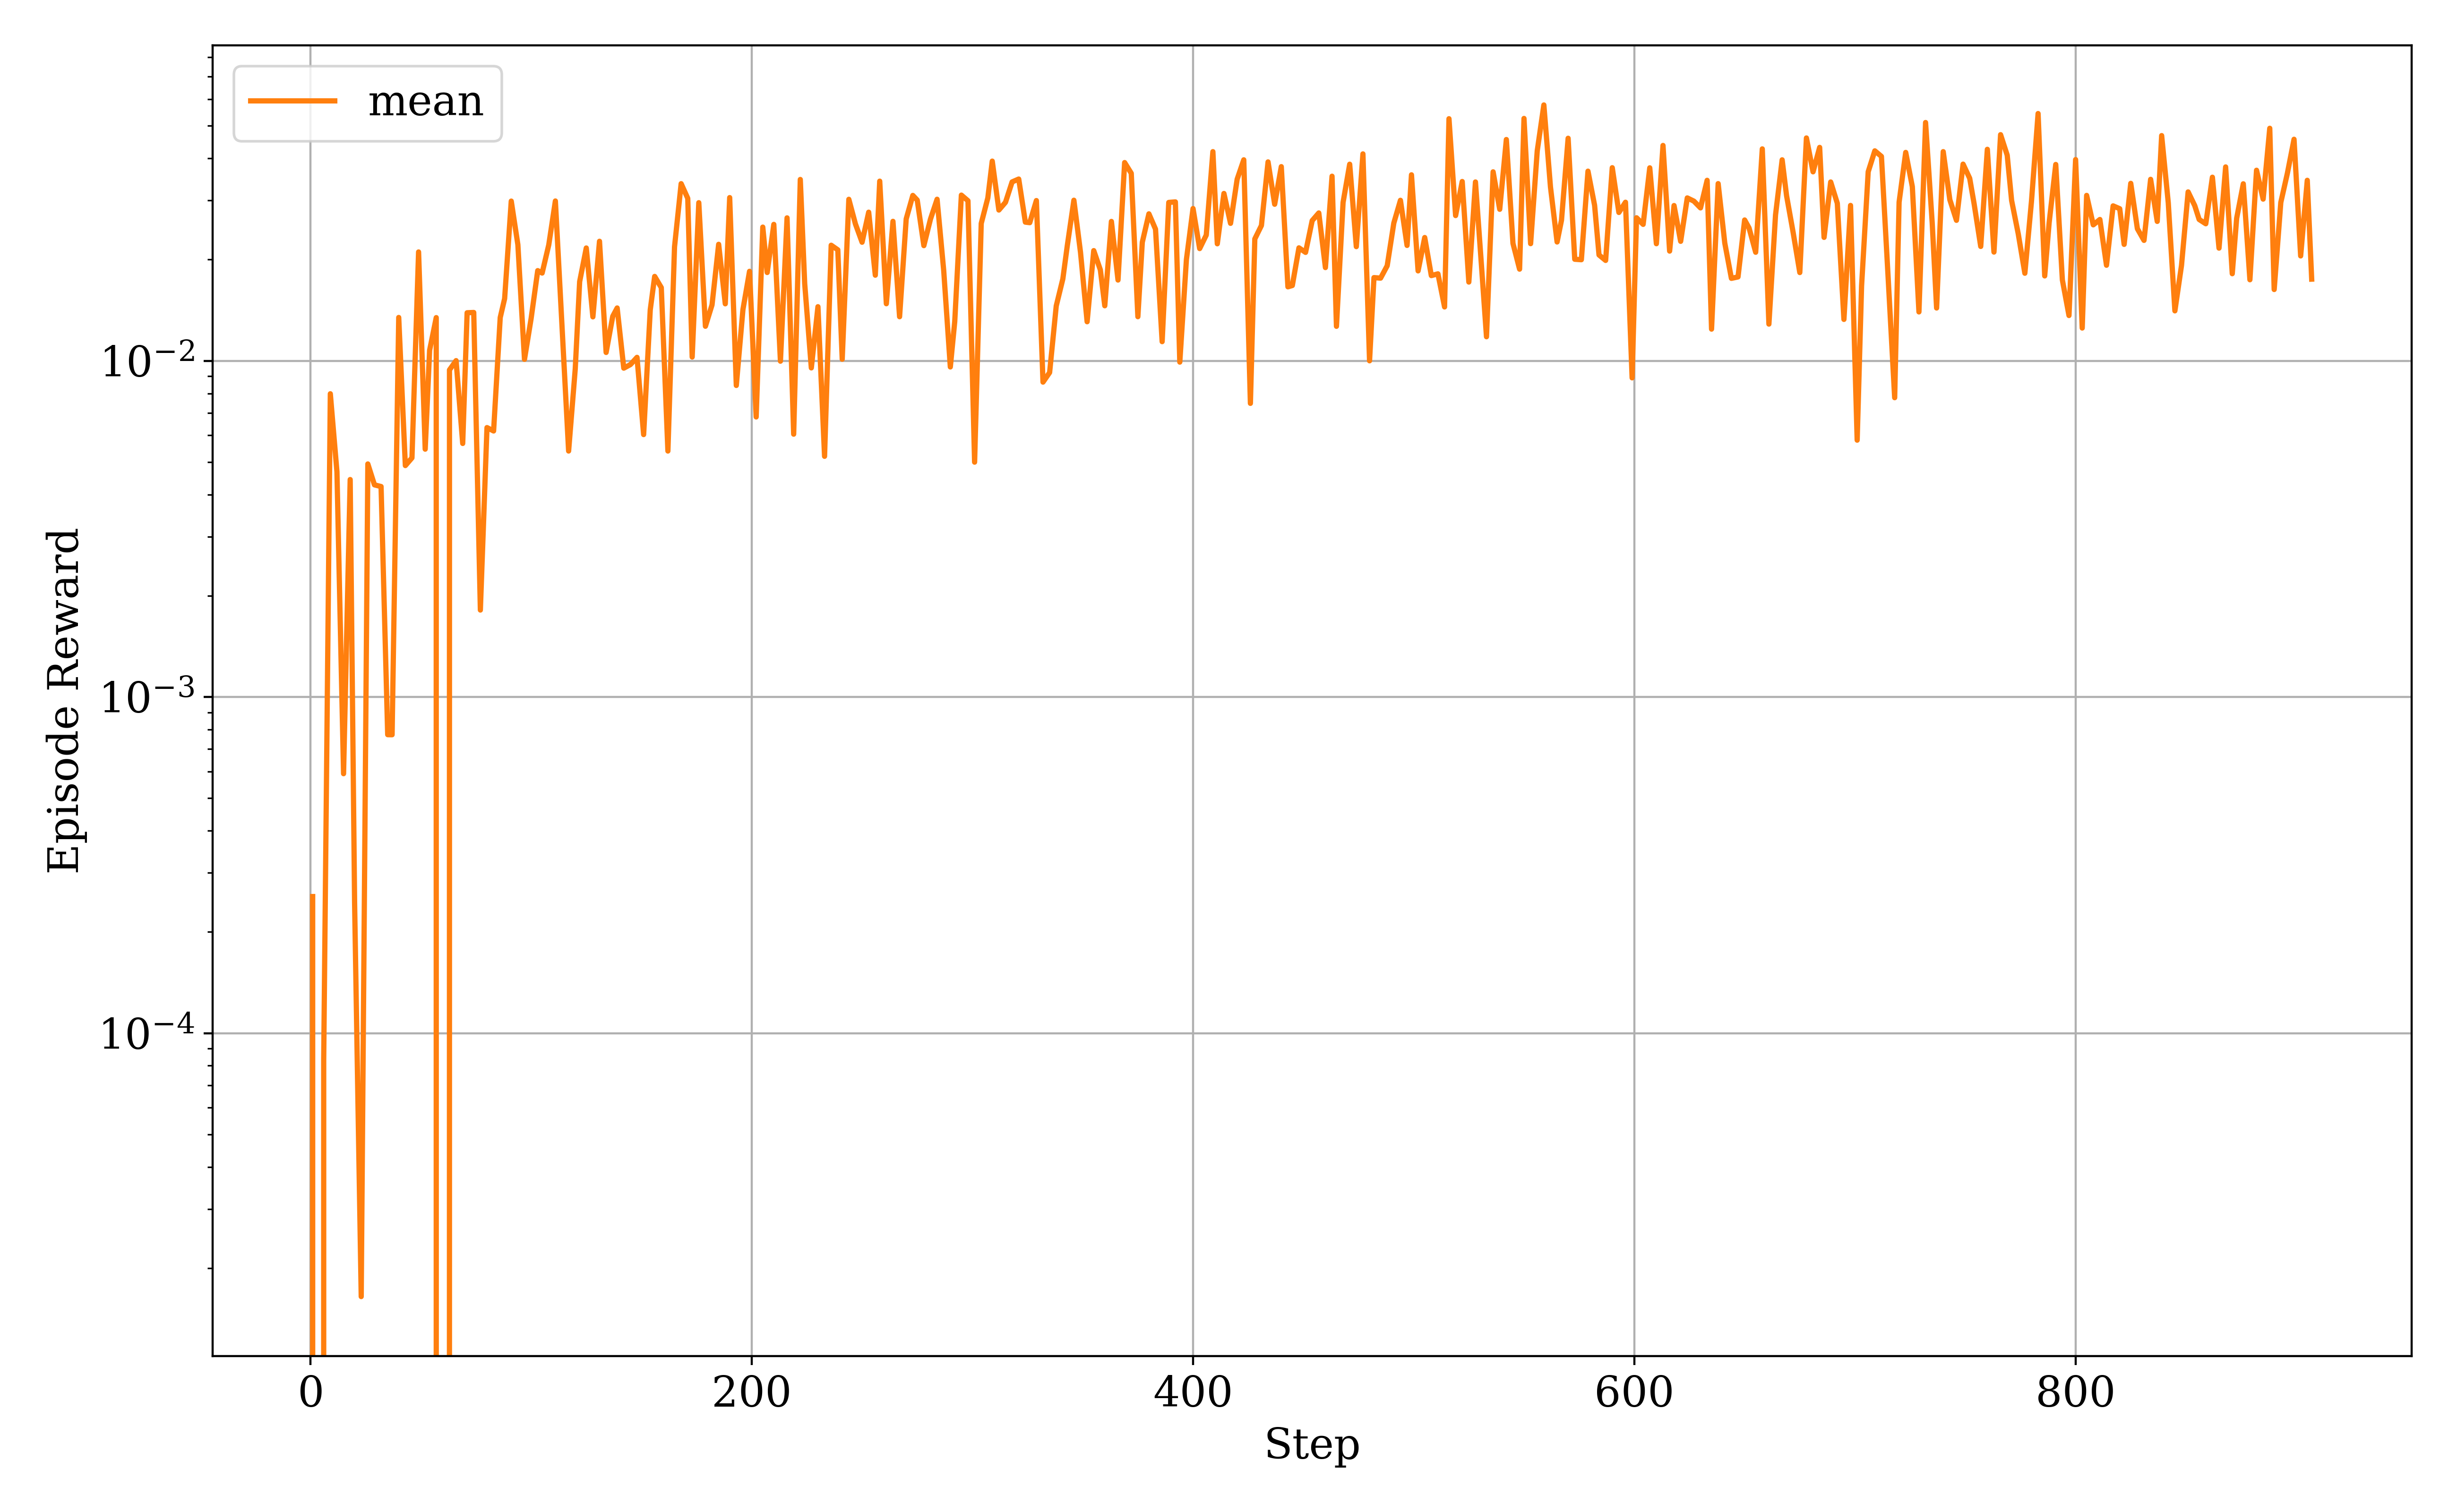
\includegraphics[width=0.85\textwidth]{Cap5/plot_random.png}
    \caption{Per-generation mean episode reward (log scale) for Run~A in
    Table~\ref{tab:smoke_config} (\texttt{InitMode.RANDOM}, 900 generations).
    The policy exhibits no
    consistent upward trend, confirming that flat random initialization provides
    insufficient learning signal in the sparse goal-scoring setting.}
    \label{fig:plot_random}
\end{figure}

In the second run, episodes began from the standard kickoff formation with small
random jitter (\texttt{InitMode.KICKOFF}), which places the ball at the centre
and the robots near their starting positions.  The per-generation mean and
minimum reward over 123 generations are shown in
Figure~\ref{fig:plot_kickoff}.  Here the policy improves rapidly: mean reward
is near zero for the first 50 generations and then rises steeply, reaching
approximately 2.0 by generation 120 — a value corresponding to consistent
multi-goal episodes.  The minimum reward tracks near zero throughout, indicating
that some environments within the batch fail to score while the mean is already
high, which is expected early in training when exploration varies widely across
parallel instances.

\begin{figure}[ht]
    \centering
    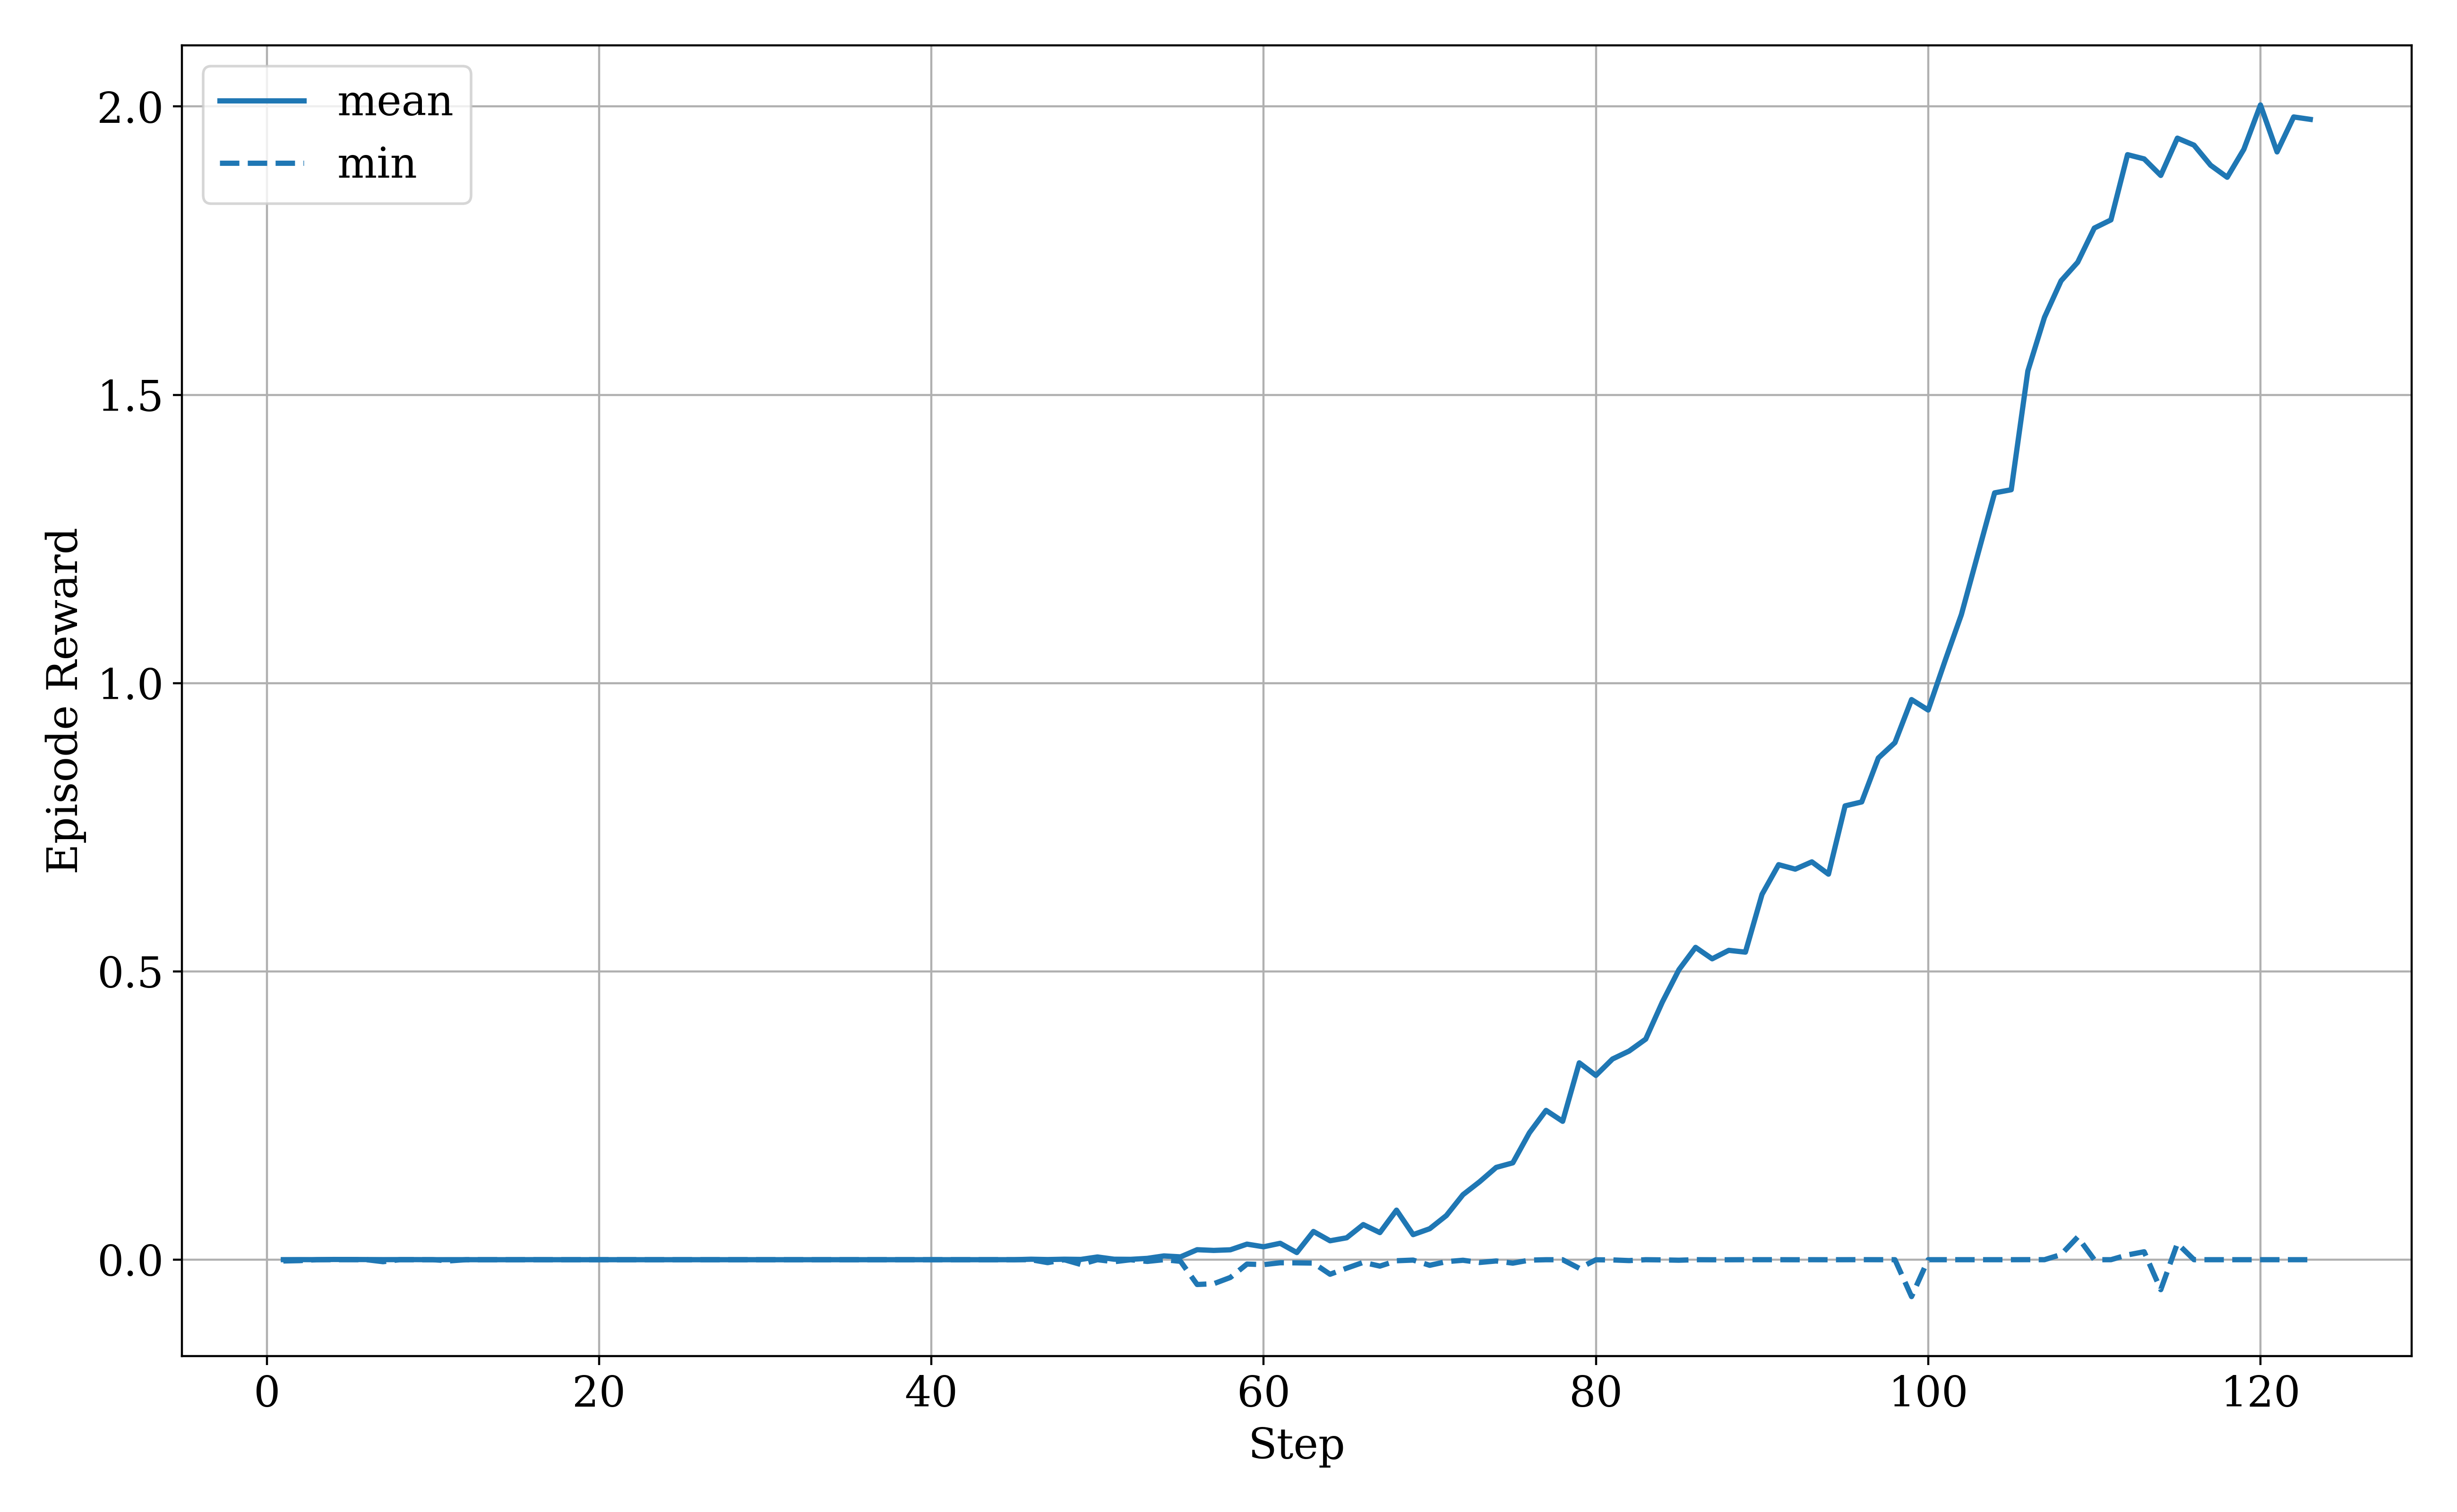
\includegraphics[width=0.85\textwidth]{Cap5/plot_kickoff.png}
    \caption{Per-generation mean and minimum episode reward for Run~B in
    Table~\ref{tab:smoke_config} (\texttt{InitMode.KICKOFF}, 123 generations).
    The policy converges rapidly
    once learning begins around generation 60, validating that the end-to-end
    training loop operates correctly under structured initialization.}
    \label{fig:plot_kickoff}
\end{figure}

Taken together, the two runs validate the training infrastructure and
simultaneously motivate the prioritized-level-replay curriculum planned for
TG-2.  Kickoff initialization is sufficient to confirm that the \gls{ppo} loop
works, but it does not cover the diversity of game states the policy must handle.
Random initialization covers that diversity but provides too sparse a signal to
drive learning.  The \gls{plr} sampler is designed precisely to interpolate
between these extremes: adaptively steering the distribution of initial states
toward configurations where the current policy's value-prediction error is
largest, thereby ensuring both sufficient difficulty and sufficient density of
learning signal throughout training.

% ==================================================================
\section{Future Planned Results}
\label{sec:future_planned_results}
% ==================================================================

The infrastructure validated above is the foundation for the experiments
planned for TG-2.  This section states what those experiments are and what each
is intended to show.

\subsection{Closing the throughput gap with a JAX-native learner.}
The throughput measurements identified two ceilings: the Gymnasium boundary and
the CPU-bound PyTorch updates of SB3.  Both stem from the learner living outside
the accelerator.  The planned remedy is a fully JAX-resident training path, in
which the policy, the rollout collection, and the gradient updates all execute
on device alongside the simulator, removing the per-step host transfers
entirely.  The target is to bring end-to-end \gls{ppo} throughput close to the
raw batched-kernel ceiling — on the order of $9 \times 10^{5}$ steps per second
on the RTX~3060, against the present $\sim 10^{4}$ of the SB3 path.  The expected
result is a before/after throughput comparison of the full training loop, not
merely the simulator in isolation.

\subsection{Prioritized-level-replay sample efficiency.}
With the sampler integrated, the central evaluation is whether prioritizing
high-learning-potential scenarios improves sample efficiency relative to uniform
initialization.  The planned result is a set of learning curves (reward and goal
rate versus environment steps) comparing the \gls{plr} sampler against a uniform
baseline under identical compute budgets, accompanied by qualitative inspection
of which scenarios the sampler prioritizes over the course of training.

\subsection{Two-stage curriculum and self-play.}
The opponents are currently stationary.  TG-2 will introduce the second
curriculum stage, replacing them with self-play opponents drawn from a history
of past policies, and will evaluate the effect of the opponent-sampling scheme
on the robustness of the learned team.  The planned result is a comparison of
policies trained with and without the curriculum, and with different
opponent-sampling strategies.

\subsection{Symmetry exploitation.}
TG-2 will quantify the benefit of the permutation- and reflection-symmetry
mechanisms described in Chapter~4, through an ablation comparing training with
and without symmetry-aware parameter sharing and data augmentation.

\subsection{Evaluation against the classical strategy.}
Finally, the trained team will be evaluated against the ITAndroids classical
strategy stack, reporting win rate, goal difference, and qualitative behavioral
analysis — the measure of whether a learned 3v3 team policy is competitive with
the hand-engineered baseline.  Sim-to-real considerations (domain randomization,
noise injection) frame this evaluation as a step toward eventual deployment, the
longer-term goal beyond TG-2.